\documentclass[12pt]{article}

% a template that a friend gave, it's worked well enough for me
% i have added some packages and stuff that have proved useful

\usepackage{fancyhdr}
\usepackage{tipa}
\usepackage{fontspec}
\usepackage{amsfonts}
\usepackage{enumitem}
\usepackage[margin=1in]{geometry}
\usepackage{graphicx}
\usepackage{float}
\usepackage{amsmath}
\usepackage{braket}
\usepackage{amssymb}
\usepackage{booktabs}
\usepackage{hyperref}
\usepackage{mathtools}
\usepackage{xcolor}
\usepackage{float}
\usepackage{algpseudocodex}
\usepackage{titlesec}
\usepackage{bbm}

\pagestyle{fancy}
\fancyhf{} % sets both header and footer to nothing
\lhead{Kevin Sheng}
\setmainfont{Comic Neue}
\renewcommand{\headrulewidth}{1pt}
\setlength{\headheight}{0.75in}
\setlength{\oddsidemargin}{0in}
\setlength{\evensidemargin}{0in}
\setlength{\voffset}{-.5in}
\setlength{\headsep}{10pt}
\setlength{\textwidth}{6.5in}
\setlength{\headwidth}{6.5in}
\setlength{\textheight}{8in}
\renewcommand{\headrulewidth}{0.5pt}
\renewcommand{\footrulewidth}{0.3pt}
\setlength{\textwidth}{6.5in}
\usepackage{setspace}
\usepackage{multicol}
\usepackage{float}
\setlength{\columnsep}{1cm}
\setlength\parindent{24pt}
\usepackage [english]{babel}
\usepackage [autostyle, english = american]{csquotes}
\MakeOuterQuote{"}

\setlength{\parskip}{6pt}
\setlength{\parindent}{0pt}

\titlespacing\section{0pt}{12pt plus 4pt minus 2pt}{0pt plus 2pt minus 2pt}
\titlespacing\subsection{0pt}{12pt plus 4pt minus 2pt}{0pt plus 2pt minus 2pt}
\titlespacing\subsubsection{0pt}{12pt plus 4pt minus 2pt}{0pt plus 2pt minus 2pt}

\hypersetup{colorlinks=true, urlcolor=blue}

\newcommand{\correction}[1]{\textcolor{red}{#1}}


\rhead{ECE 236A}

\newcommand*{\vertbar}{\rule[-1ex]{0.5pt}{2.5ex}}
\newcommand*{\horzbar}{\rule[.5ex]{2.5ex}{0.5pt}}

\begin{document}

\begin{enumerate}
      \item Let us progressively subtract scalar multiples of permutation matrices
            from the doubly stochastic matrix $M$ until we end up with the zero matrix.

            If we can always find a permutation matrix $P$ s.t. $P_{ij} \ne 0 \to M_{ij} \ne 0$,
            we subtract $m \cdot P$, where $m=\min_{i, j, P_{ij} \ne 0} M_{ij}$.
            We keep on doing this until we arrive at the zero matrix.

            To show that we can always find such a $P$, notice
            that we can treat the matrix as a bipartite graph, where $M_{ij}$
            is the weight from node $i$ on one side to node $j$ on the other.
            Similarly, any permutation matrix can be thought of as a
            perfect matching on a bipartite graph, since each row is "matched"
            with exactly one column and vice versa.

            Notice that if we construct a flow graph out of this,
            our max flow will be exactly $n$.
            Since the sum of the outgoing edges from each node on one side is $1$
            and the sum of incoming edges to each node on the other side is also $1$,
            we can send exactly $1$ unit across all edges on the source.

            To turn this into a matching, we change all edges with
            \textit{nonzero} capacity into $1$ and run max flow.
            This will certainly not decrease the possible flow while
            turning the result into a valid perfect bipartite matching.

            After subtracing $m \cdot P$ from the matrix,
            we can then scale it by $\frac{1}{1-m}$ to make the sum of the rows
            and columns again.
            This is possible because the sum of each row and column
            is decreased by exactly $m$ due to the properties of the permutation matrix.

            Now after having performed enough operations to reduce the matrix
            to all zeros, we just have to prove that this is a convex combination.
            To do this, notice that at each step the total sum of the actual
            matrix reduces by $mn$.
            Combined with that we end up with the zero matrix,
            \[\sum_{\text{all ops}} mn=n \therefore \sum_{\text{all ops}} m=1 \eqno\square\]
      \item \begin{enumerate}
                  \item We start with $\vec{0}$:
                        \[\begin{array}{c|rr|l}
                                        & x  & y  & \mathbf{1} \\ \hline
                                    c_1 & -1 & 1  & 4          \\
                                    c_2 & -1 & -1 & 6          \\ \hline
                                        & 1  & -1 & 0          \\
                              \end{array}\]
                        The only valid entering variable is $y$,
                        so we increase it as much as possible until $c_2$ blocks it at $y=6$.
                        \[\begin{array}{c|rr|l}
                                        & x  & c_2 & \mathbf{1} \\ \hline
                                    c_1 & -2 & -1  & 10         \\
                                    y   & -1 & -1  & 6          \\ \hline
                                        & 2  & 1   & -6         \\
                              \end{array}\]
                        There's no more negative numbers in the bottom row, so
                        our optimal solution is $z=-6$ at $x=0$ and $y=6$.
                  \item 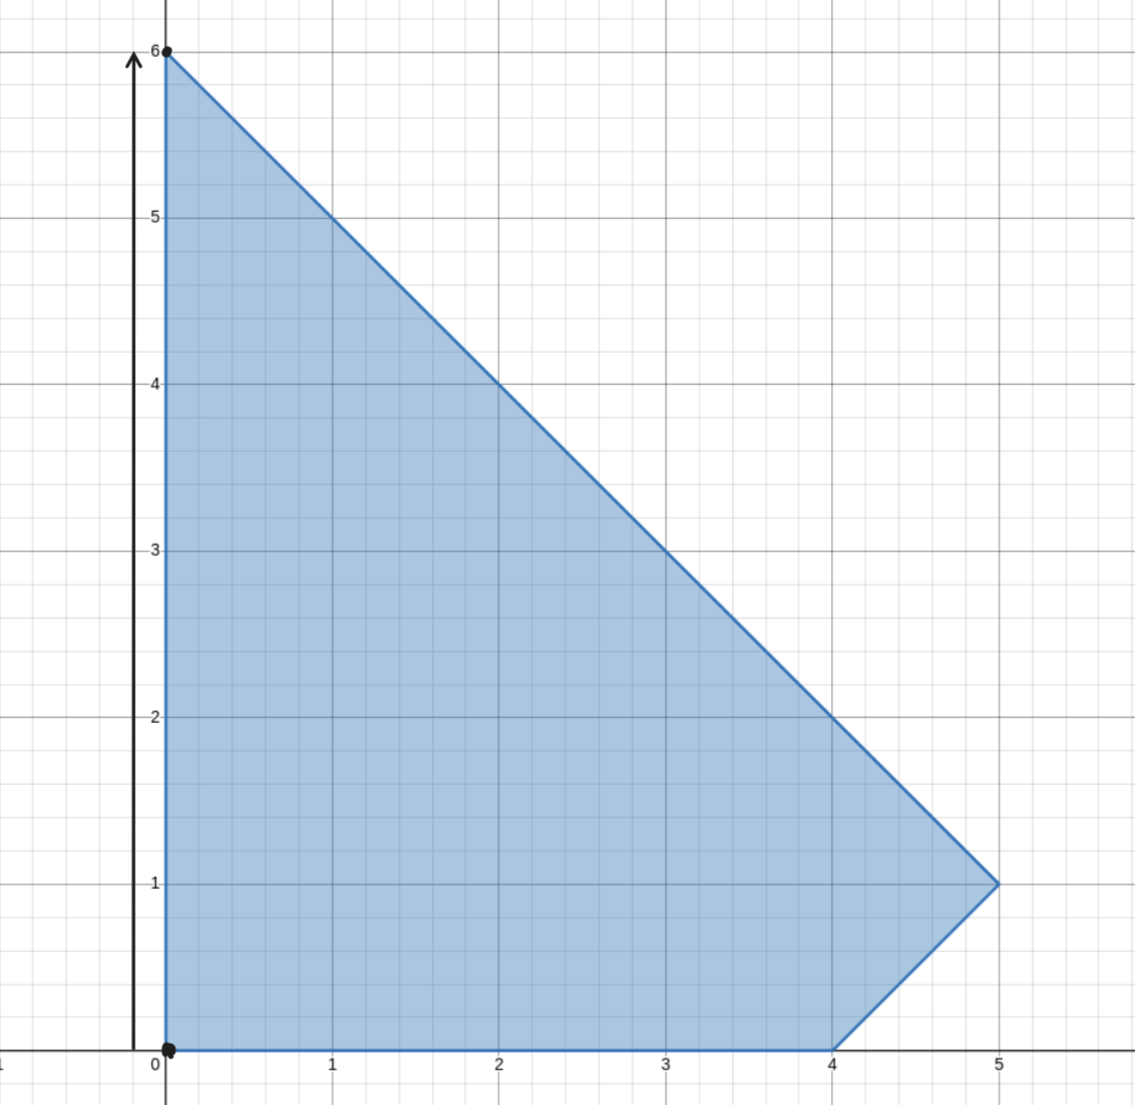
\includegraphics[width=12cm]{img/hw5/simplex_path}
                  \item We start with the same tableau, only with a different bottom row:
                        \[\begin{array}{c|rr|l}
                                        & x  & y  & \mathbf{1} \\ \hline
                                    c_1 & -1 & 1  & 4          \\
                                    c_2 & -1 & -1 & 6          \\ \hline
                                        & -1 & 1  & 0          \\
                              \end{array}\]
                        In this case, $x$ is entering and $c_1$ is blocking when $x=4$.
                        \[\begin{array}{c|rr|l}
                                        & c_1 & y  & \mathbf{1} \\ \hline
                                    x   & -1  & 1  & 4          \\
                                    c_2 & 1   & -2 & 2          \\ \hline
                                        & 1   & 0  & -4         \\
                              \end{array}\]
                        So our optimal value is $z=-4$, but we can increase $y$ at no cost.
                        This gives us the two vertices $(4, 0)$ and $(5, 1)$.
                        Our optimal set is thus
                        \[\left\{\begin{pmatrix}x \\ y\end{pmatrix}\,
                              \middle|\, x=y+4, 0 \le y \le 1\right\}\]
                  \item Initial tableau:
                        \[\begin{array}{c|rr|l}
                                        & x  & y  & \mathbf{1} \\ \hline
                                    c_1 & 2  & -1 & 2          \\
                                    c_2 & -1 & 1  & 1          \\ \hline
                                        & -1 & -1 & 0          \\
                              \end{array}\]
                        Choose $x$ as our entering variable.
                        $c_2$ blocks it at $x=1$:
                        \[\begin{array}{c|rr|l}
                                        & c_2 & y  & \mathbf{1} \\ \hline
                                    c_1 & -2  & 1  & 4          \\
                                    x   & -1  & 1  & 1          \\ \hline
                                        & 1   & -2 & -1         \\
                              \end{array}\]
                        As we can see, $y$ and the objective function can be made
                        arbitrarily small since there's no negative values in its column.
                        Thus, this problem is unbounded.

                        The path is below: \\
                        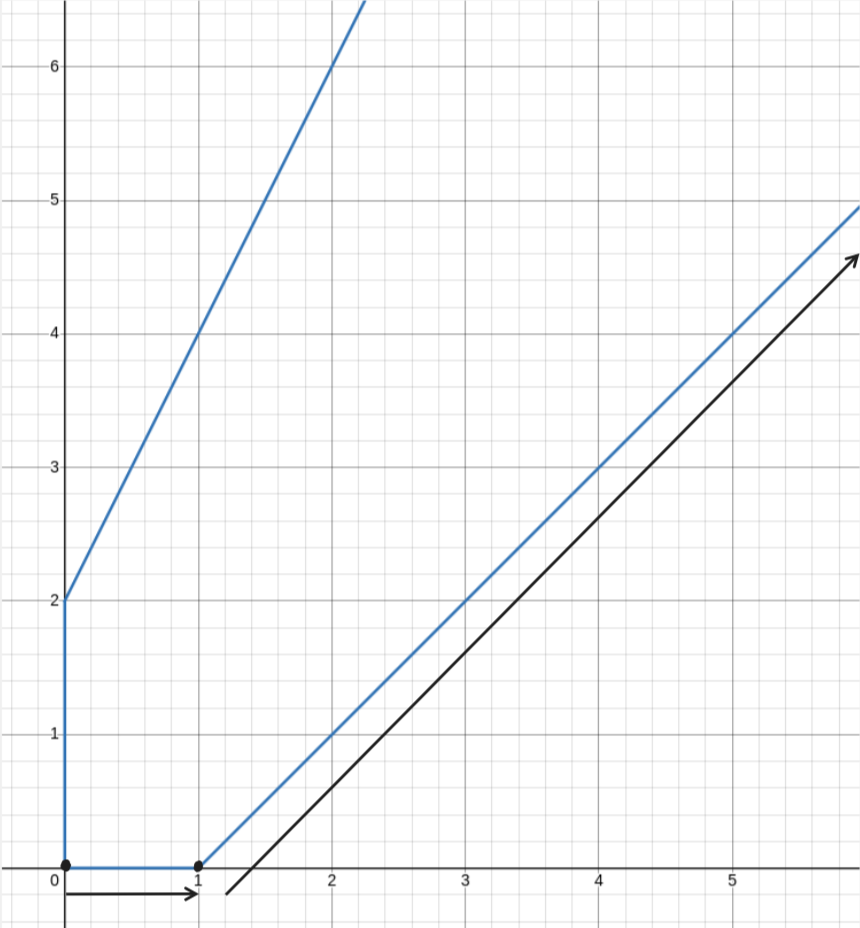
\includegraphics[width=12cm]{img/hw5/unbounded_path}
            \end{enumerate}
      \item Notice that $x_3$ functions as nothing more than a slack variable.
            The sum of $x_1$ and $x_2$ just has to be greater than $\frac{1}{2}$,
            and $x_3$ can fill in the rest to meet the equality.

            I'll name the constraints as follows:
            \begin{gather*}
                  c_1=-x_1+\frac{1}{2} \ge 0 \\
                  c_2=-x_2+\frac{1}{2} \ge 0 \\
                  c_3=x_1+x_2-\frac{1}{2} \ge 0 \\
            \end{gather*}
            We start with
            \[\begin{array}{c|rr|l}
                            & c_1 & c_2 & \mathbf{1}  \\ \hline
                        x_1 & -1  & 0   & \frac{1}{2} \\
                        x_2 & 0   & -1  & \frac{1}{2} \\
                        c_3 & -1  & -1  & \frac{1}{2} \\ \hline
                            & -1  & 1   & 0           \\
                  \end{array}\]
            Only $c_1$ is available to pivot; $x_1$ and $c_3$ block it at $c_1=\frac{1}{2}$.
            Arbitrarily choosing $x_1$ as the blocker, we get
            \[\begin{array}{c|rr|l}
                            & x_1 & c_2 & \mathbf{1}   \\ \hline
                        c_1 & -1  & 0   & \frac{1}{2}  \\
                        x_2 & 0   & -1  & \frac{1}{2}  \\
                        c_3 & 1  & -1  & 0            \\ \hline
                            & 1  & 1   & -\frac{1}{2} \\
                  \end{array}\]
            There's nowhere to go now, so our optimal value is $z=\frac{1}{2}$
            at $x_1=0, x_2=\frac{1}{2}, x_3=\frac{1}{2}$.

            \pagebreak

      \item \begin{enumerate}
                  \item I won't put $p$ into the tableau since this LP is supposed to be infeasible:
                        \[\begin{array}{c|rrr|l}
                                        & x_1 & x_2 & x_0 & \mathbf{1} \\ \hline
                                    c_1 & -1  & -1  & 0   & 1          \\
                                    c_2 & -2  & 1   & 1   & -2         \\ \hline
                                    z_0 & 0   & 0   & 1   & 0          \\
                              \end{array}\]
                        Pivotting so that $x_0=2$ gives us
                        \[\begin{array}{c|rrr|l}
                                        & x_1 & x_2 & c_2 & \mathbf{1} \\ \hline
                                    c_1 & -1  & -1  & 0   & 1          \\
                                    x_0 & 2   & -1  & 1   & 2          \\ \hline
                                    z_0 & 2   & -1  & 1   & 2          \\
                              \end{array}\]
                        Now we choose $x_2$ to enter.
                        $c_1$ blocks it at $x_2=1$, so our new tableau is
                        \[\begin{array}{c|rrr|l}
                                        & x_1 & c_1 & c_2 & \mathbf{1} \\ \hline
                                    x_2 & -1  & -1  & 0   & 1          \\
                                    x_0 & 3   & 1   & 1   & 2          \\ \hline
                                    z_0 & 3   & 1   & 1   & 1          \\
                              \end{array}\]
                        As we can see, the optimal value is $x_0=1$, proving the original LP infeasible. $\square$
                  \item Starting with
                        \[\begin{array}{c|rrr|l}
                                        & x_1 & x_2 & x_0 & \mathbf{1} \\ \hline
                                    c_1 & 2   & -1  & 1   & -1         \\
                                    c_2 & 1   & 2   & 1   & -2         \\ \hline
                                    z   & -2  & 1   & 0   & 0          \\ \hline
                                    z_0 & 0   & 0   & 1   & 0          \\
                              \end{array}\]
                        We do a special pivot to set $x_0=2$ and get
                        \[\begin{array}{c|rrr|l}
                                        & x_1 & x_2 & c_2 & \mathbf{1} \\ \hline
                                    c_1 & 1   & -3  & 1   & 1          \\
                                    x_0 & -1  & -2  & 1   & 2          \\ \hline
                                    z   & -2  & 1   & 0   & 0          \\ \hline
                                    z_0 & -1  & -2  & 1   & 2          \\
                              \end{array}\]
                        Then we can pivot $x_1$ which $x_0$ blocks at $x_1=2$:
                        \[\begin{array}{c|rrr|l}
                                        & x_0 & x_2 & c_2 & \mathbf{1} \\ \hline
                                    c_1 & -1  & -5  & 2   & 3          \\
                                    x_1 & -1  & -2  & 1   & 2          \\ \hline
                                    z   & 2   & 5   & -2  & -4         \\ \hline
                                    z_0 & 1   & 2   & 0   & 0          \\
                              \end{array}\]
                        We've hit $x_0=0$, so we can start reducing the actual objective function.
                        Notice, though, that if we choose $c_2$ as our entering variable,
                        we can decrease the objective function arbitrarily,
                        since there's no negative entries in its column.
                        Thus, this problem is unbounded. $\square$
            \end{enumerate}
      \item \begin{enumerate}
                  \item \begin{enumerate}
                              \item No, because $e_1+e_2$ literally isn't feasible.
                              \item No, because simplex could have chosen $e_2+e_4$,
                                    a better vertex.
                              \item Yes.
                                    Simplex could have chosen $x_2$ then $x_4$ as entering variables.
                              \item Yes.
                                    Simplex could have chosen $x_3$ then $x_4$ as entering variables.
                                    $x_3$ goes to $0$ when we increase $x_4$
                                    since at that point it's in a row and a constraint mandates that $x_3+x_4 \le 1$.
                        \end{enumerate}
                  \item No.
                        Simplex has to constantly improve the objective function with each pivot,
                        so if such a $c$ were to exist we'd need it to satisfy
                        \[0 < c_1 < c_1 + c_3 < c_3\]
                        From this we can see that we need $0<c_1$ and $0>c_1$, which is a contradiction.
            \end{enumerate}
\end{enumerate}
\end{document}
